\documentclass{article}

\usepackage[utf8]{inputenc}
\usepackage{graphicx}
\usepackage{amsmath}
\usepackage{amsfonts}
\usepackage{amssymb}
\usepackage{comment}
\usepackage{geometry}
\usepackage{float}
\usepackage{caption}
\usepackage{subcaption}
\usepackage{listings}

\geometry{a4paper, margin=1in}

\lstset{
    basicstyle=\ttfamily\small,
}

\title{CSCE 312 - Lab 1}
\author{Kevin Lei}
\date{\today}


\begin{document}

\maketitle

\begin{comment}
\begin{abstract}
The purpose of this lab is to introduce low-level system design.
\end{abstract}
\end{comment}

\section{Problem 1}

\subsection{Part A}
\textbf{Tag 1: } The purpose of this code is to make sure that the file is open, or the point to the file is not null. 
If the file is not open, then the program will exit.\\
\textbf{Tag 2: } This code calls the \lstinline!gettimeofday()! function from the \lstinline!time.h! header.
It then assigns the value to the \lstinline!this_instant! variable which is passed by reference. \\
\textbf{Tag 3: } This line of code writes the int data type size in bits and bytes to the output file. \\
\textbf{Tag 4: } This line does the same as Tag 3 except it writes to the console instead of a file. \\

\subsection{Part B}
\begin{figure}[H]
    \centering
    
\includegraphics[width=0.75\textwidth]{./images/prob1partb.png}
    \caption{Compiling and running \lstinline!lab1_prob1.c!}
\end{figure}

\subsection{Part C}
The \lstinline!timeval! struct contains the \lstinline!tv_sec! variable, which is a numeric value like int or double.

\section{Problem 2}

\subsection{Part A}
\begin{figure}[H]
    \centering
    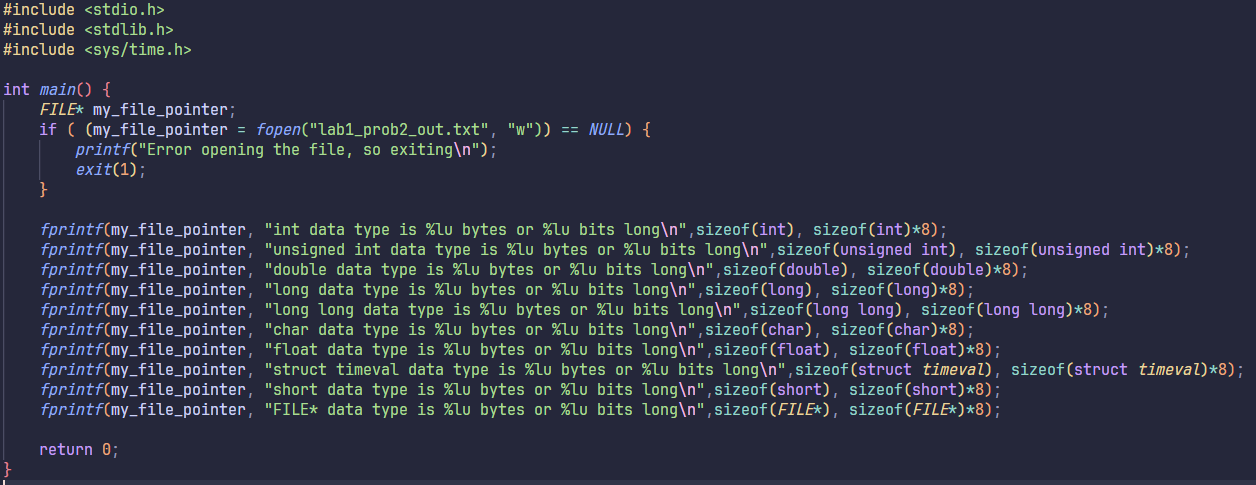
\includegraphics[width=1\textwidth]{./images/prob2parta1.png}
    \caption{Source code for \lstinline!lab1_prob2.c!}
\end{figure}

\begin{figure}[H]
    \centering
    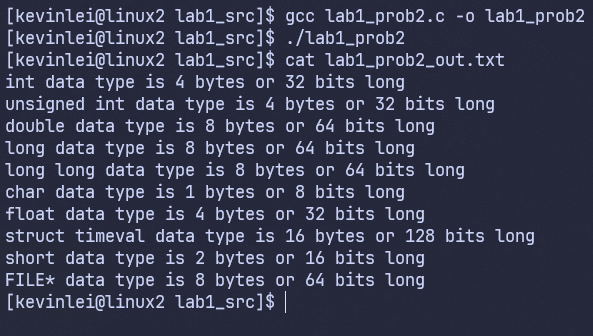
\includegraphics[width=0.75\textwidth]{./images/prob2parta2.png}
    \caption{Compiling and running \lstinline!lab1_prob2.c!, including the output.}
\end{figure}

\subsection{Part B}
memory alignment lmao

\section{Problem 3}

\section{Problem 4}

\section{Problem 5}


\begin{comment}
\section{Materials and Methods}
This section should detail the materials used in the experiment and the methods followed. Be specific enough that someone could replicate your experiment using this section.

\subsection{Materials}
List all the materials used in the experiment.

\subsection{Methods}
Detail the procedures you followed in the experiment.

\section{Results}
Present the results of your experiment. Use tables, graphs, and figures where appropriate. Make sure all visuals are well-labelled and include captions.

\begin{figure}[H]
\centering
\includegraphics[width=0.5\textwidth]{image_name.png}
\caption{Caption for the image.}
\end{figure}

\section{Discussion}
Analyze the results of the experiment. Discuss whether the results support your hypothesis or not. Discuss any errors or anomalies you encountered and how they may have affected the results.

\section{Conclusion}
Summarize the findings of the experiment and their implications. Discuss what this experiment contributes to the field, and suggest any future research that may be necessary or interesting.

\section{References}
List all references used in your report. Make sure to follow a consistent and appropriate citation style.

\end{comment}

\end{document}
